\subsection{Deep Ensembles (\cite{fort2019ensemble})}

So you have a dataset of $x\in\mathbb{R}^d$ and try to predict $y$.
If you build a neural network to predict it and make an ensemble from them.
You can input $x$ to all models and aggregate output. For example, mean averaging.

Imaging your neural net has only single weight.
After you optimize you get somewhere on axis.
So you fit to the best training accuracy.
There are different picks of top accuracies.

What if we create a model that will capture all distribution of possible weights (Fig. \ref{fig:space_solutions})

\begin{figure}[h]
    \centering
    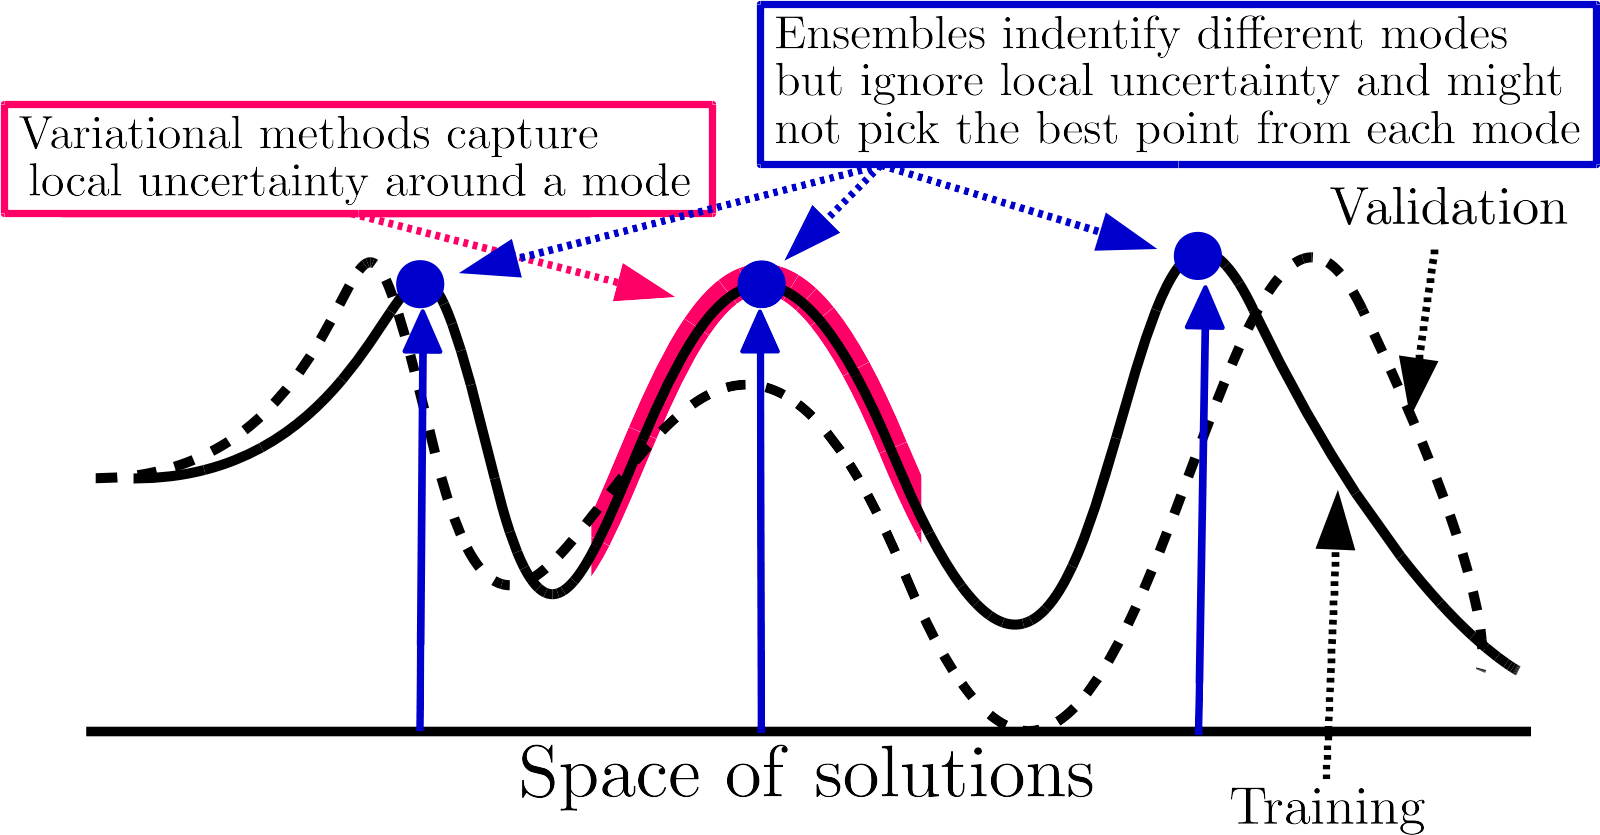
\includegraphics[width=0.3\textwidth]{images/space_solutions.png}
    \caption{Space solutions}
    \label{fig:space_solutions}
\end{figure}

What they did? They look into training trajectory of the single run.
This paper is half about ensembling and half about the training process.
The first thing is we have a random initialization. We do gradient descent and reach local minina.
You repeat a process with different random initialization point.
The question is do these local minimas describe the same optimal functions or are they fundementally different functions that just happend to reach same accuracy.

